\section{Results}
\subsection{Detection and alarm burden}
The primary improvement criterion failed. Fixed return alarmed on 2,778 benign observations (4.68\%), compared with 2,452 (4.13\%) for fused hysteresis: a \RelativeIncrease\% increase rather than the required reduction. It reduced benign points by 59.41\% against mode hysteresis, which was insufficient because the criterion required improvement against both controls. The candidate had 41 benign alarm episodes versus 45 for fused hysteresis and 175 for mode hysteresis. Its longer alarm time therefore did not imply more alarm episodes.

\begin{table}[htbp]\centering\small
\caption{Selected controls and candidate on the fresh pooled population. Overlap/fresh counts have denominator 90; early denotes events with premature clearing. Full roster appears in Appendix~\ref{app:all}.}
\begin{tabular}{lrrrr}
\toprule
Method & Benign (\%) & F1 & Overlap/fresh & Early \\
\midrule
ARX(4) & 6.00 & 0.644 & 90/80 & 90 \\
Rolling mean (45) & 4.43 & 0.709 & 90/72 & 87 \\
CUSUM & 44.05 & 0.216 & 81/39 & 0 \\
Following hysteresis & 2.57 & 0.795 & 90/72 & 90 \\
Fused hysteresis & 4.13 & 0.677 & 90/72 & 3 \\
Mode hysteresis & 11.52 & 0.519 & 90/72 & 0 \\
Fixed return & 4.68 & 0.650 & 90/72 & 0 \\
\bottomrule
\end{tabular}
\label{tab:main}
\end{table}

Fixed return, fused hysteresis and mode hysteresis each overlapped all 90 events and produced 72 fresh event onsets. All 18 absent fresh onsets for fixed return occurred in the missing-context condition; later known overlap did not satisfy the stricter fresh-onset definition. The candidate had no premature clears or known unalarmed gaps before declared return. Fused hysteresis had premature clearing in three events and 15 gap observations. All 90 candidate events returned and cleared within five seconds; the maximum measured clearing delay was 0.92 s. 

Following-error hysteresis had fewer benign alarms and higher command-interval F1: F1 was 0.795, versus 0.650 for fixed return, with 1,529 benign alarm points. It nevertheless cleared before declared physical return in all 90 events. Its zero maximum clearing delay reflects alarms already absent at return. Retaining evidence after command restoration counts against command-interval precision even when it aligns with the separate return diagnostic. Fixed return had 10,188 alarmed observations in the common 22,500-observation post-command windows, compared with 9,144 for fused hysteresis and 4,187 for following hysteresis.

CUSUM overlapped 81 events with 39 fresh onsets, missed nine events, and alarmed on 26,165 benign observations. None of its 81 detected-returned events cleared within the five-second window. The rolling mean remained a useful control with F1 0.709 and 2,632 benign alarm points, while showing premature clearing in 87 events. Persistence and AR had low point recall despite many event overlaps; their alarms often captured transitions rather than sustained deviation. 

\begin{figure}[htbp]\centering
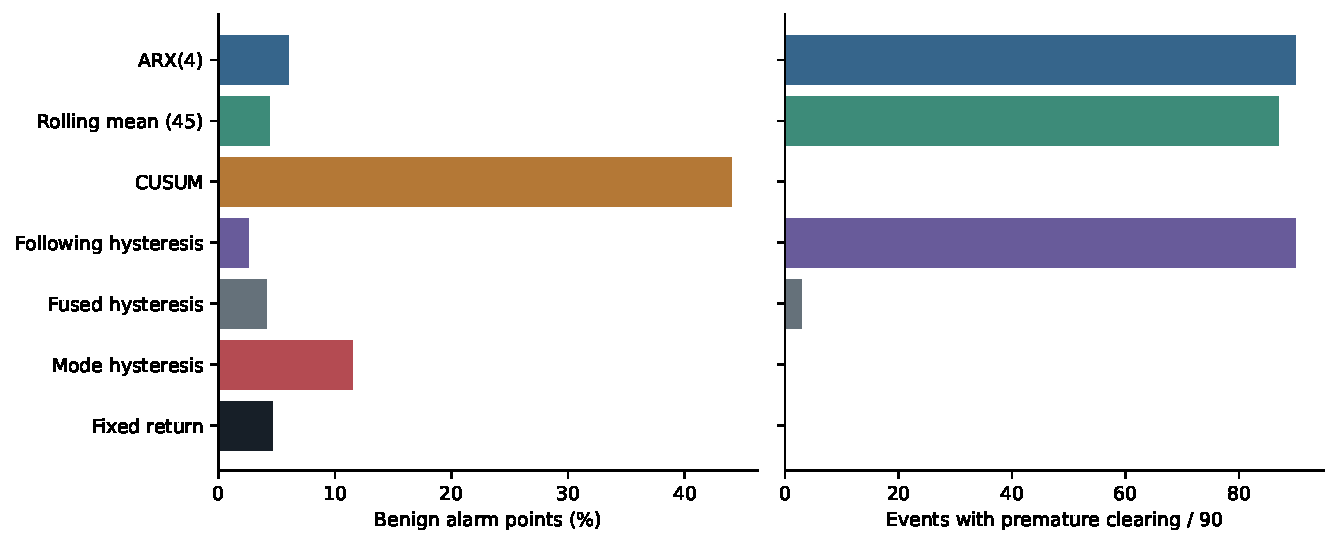
\includegraphics[width=\linewidth]{figures/tradeoff.pdf}
\caption{Benign alarm time and premature clearing describe different costs. All panels use saved pooled outcomes; zero premature clearing alone can also describe a method that remains alarmed. }
\label{fig:tradeoff}
\end{figure}

\subsection{Component ablations}
At the candidate's identical entry threshold, ordinary hysteresis had five premature-clear events, one-sample fixed return had 44, and removing the noise margin had one. The full rule had none (Table~\ref{tab:matched}). Removing the dwell reduced benign alarms from 2,778 to 1,813; removing the margin reduced them to 2,486. Both components reduced premature clearing while increasing benign alarm time.

\begin{table}[htbp]\centering\small
\caption{Matched-entry component study. All rows use $h=\CandidateThreshold$. These diagnostics do not have matched calibration alarm counts.}
\begin{tabular}{lrrr}
\toprule
Decision at same entry threshold & Benign points & Early clears & F1 \\
\midrule
Fixed return & 2778 & 0 & 0.650 \\
Matched point & 1430 & 90 & 0.731 \\
Matched hysteresis & 2389 & 5 & 0.680 \\
Matched no dwell & 1813 & 44 & 0.706 \\
Matched no margin & 2486 & 1 & 0.674 \\
\bottomrule
\end{tabular}
\label{tab:matched}
\end{table}

With separate normal-only calibration, the no-dwell variant had 1,872 benign points and 44 premature-clear events; the no-margin variant had 2,488 and one. Replacing fused entry with reference-only entry yielded 2,547 benign points and no premature clearing. Replacing it with following-only entry produced exactly the same alarm and unknown arrays as the full candidate in every one of the 144 episodes. Sample-by-sample comparison confirmed this equality. Reference-based \emph{entry} therefore added no observed decision benefit. The reference continued to supply the recovery condition.

The command-reset control and fused hysteresis had identical aggregate outcomes. Their internal state trajectories were not tested for equivalence.

\subsection{Plant conditions}
All four listed stateful methods produced zero benign alarms in P1. Fixed return produced 936 in P2 and 1,842 in P3, compared with 882 and 1,570 for fused hysteresis. Mode hysteresis produced 1,102 and 5,742. Fixed return increased benign alarm points relative to fused hysteresis in both lagged plants. Increasing model discrepancy and noise co-varied across these declared strata; the experiment does not isolate the causal effect of actuator lag from the independently changed masses, damping and sensor noise.

\begin{figure}[htbp]\centering
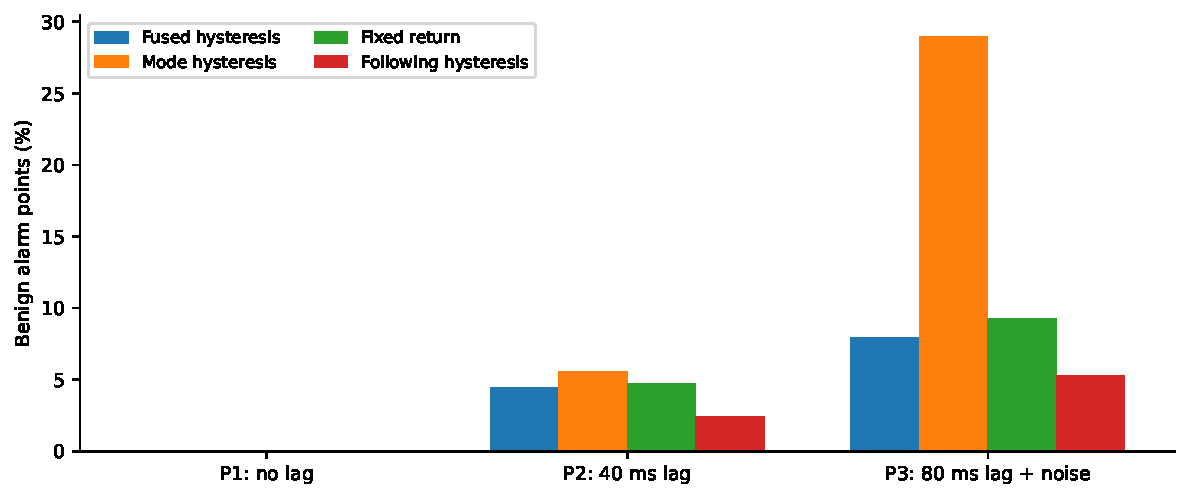
\includegraphics[width=.95\linewidth]{figures/plant_strata.pdf}
\caption{Plant-stratified benign alarm burden; each stratum contains 19,800 benign observations. Masses and damping also differ between plants, so this is not a controlled lag-only effect.}
\label{fig:strata}
\end{figure}



\subsection{Computational cost}
The supervised run completed in \Wall~s wall time and \CPU~s worker CPU time, with \RSS~MiB peak measured memory and \Output~MiB outputs. The single run completed within all resource limits. Physical generation took 17.245~s, following-observer propagation 46.921~s, shared model-bank propagation 10.073~s and score assembly 0.627~s. These are measured component totals, not independent latency estimates for each method. Model-bank work is cached across compatible episodes and includes calibration; the separately reported calibration total overlaps some of it and must not be added again.

Candidate decision replay alone took about 11.207 ms summed across all 144 saved streams, excluding prediction and scoring. Vectorized point decisions and sequential state machines have different implementation paths, so those totals are not an embedded deployment benchmark. 
